\section{Participation notes 4}
Participant: Teacher

\begin{itemize}
    \item \textbf{Have them read the code-example} - Participant mentions that participant has very limited experience with C++ in particular. 
    \item \textbf{Have them draw the structure} - 
    \item \textbf{} - User explains that there is a main procedure and two under-procedures called by main. Namespace is a concept that the user has little experience with, but draws it as a dotted line around the two sub procedures. Participant then mentions the control flow going from main to the two sub procedures. 
    \item \textbf{Have them submit the git URL} - User reads the description before clicking the submit button without content repository field. User then mentions that nothing happen when clicking submit and is unable to continue without guidance.
    \item \textbf{Have them get the main() implementation} - Participant tries to use the top bar menu and does not try the navigation within the expected time. When main is visible, the user immediately clicks it to get implementation.
    \item \textbf{Participant visualization} \includepdf[pages={7}]{inc/generalAppendix/userStudies/participantsVisualization.pdf}
\end{itemize}